\begin{center}
	\Huge
	Transformation af data
\end{center}
\section*{Linearisering af data}
\stepcounter{section}

Har vi data, vi forventer kan beskrives ved en eksponentiel model vil det være en fordel at kunne transformere datasættet, så det kan beskrives ved en lineær model. Dette gælder tilsvarende hvis vi har data, der kan beskrives ved en potensmodel. Vi kan anvende følgende sætninger, når vi skal transformere data.
\begin{setn}
	Hvis der er en eksponentiel sammenhæng mellem to variable $x$ og $y$, altså at
	\begin{align*}
		y = b\cdot a^x,
	\end{align*}
	så er der en lineær sammenhæng mellem $x$ og $\ln(y)$.
\end{setn}
\begin{proof}
	Vi har, at 
	\begin{align*}
		y = b\cdot a^x,
	\end{align*}
	så derfor gælder der, at 
	\begin{align}\label{enkeltlog}
		\ln(y) &= \ln(b\cdot a^x) \nonumber \\
		&= \ln(b) + \ln(a^x)\nonumber \\
		&= \ln(b) + x\ln(a).
	\end{align}
\end{proof}
\begin{setn}
	Hvis der er en potenssammenhæng mellem to variable $x$ og $y$, altså at
	\begin{align*}
		y = b\cdot x^a,
	\end{align*}
	så er der en lineær sammenhæng mellem $\ln(x)$ og $\ln(y)$.
\end{setn}
\begin{proof}
	Vi har, at
	\begin{align*}
		y = b\cdot x^a.
	\end{align*}
	Som før fås nu, at 
	\begin{align*}
		\ln(y) &= \ln(b \cdot x^a)\\
		&= \ln(b) + \ln(x^a)\\
		&= \ln(b) + a\ln(x).
	\end{align*}
\end{proof}

\begin{exa}
	Vi har følgende \href{https://github.com/ChristianJLex/TeachingNotes/raw/master/2022-2023/Data%20og%20lign/Bakterier.xlsx}{\color{blue!60}datasæt}, der beskriver sammenhængen mellem forløbne timer og antallet af bakterier i en opløsning. 
	Vi udfører eksponentiel regression i Maple og får regressionslinjen, der kan ses af Fig. \ref{fig:expreg}.
	\begin{figure}[H]
		\centering
		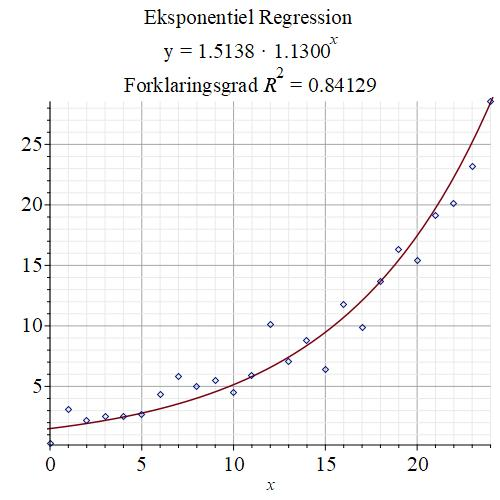
\includegraphics[width=0.7\textwidth]{Billeder/bakterieexpreg.jpg}
		\caption{Eksponentiel regression på bakteriedata}
		\label{fig:expreg}
	\end{figure}
	Vi får følgende sammenhæng mellem antallet af bakterier $y$ (i mia.) og forløbne timer $x$.
	\begin{align*}
		y = 1.5138\cdot 1.13^x.
	\end{align*}
	Vi tager $\ln$ af alle $y$-værdierne og laver i stedet lineær regression. Dette giver regressionslinjen, der kan ses af Fig. \ref{fig:linlogreg}.
	At transformere alle y-værdierne ved at tage logaritmen af dem giver os et \textit{enkeltlogaritmisk koordinatsystem}.
	\begin{figure}[H]
		\centering
		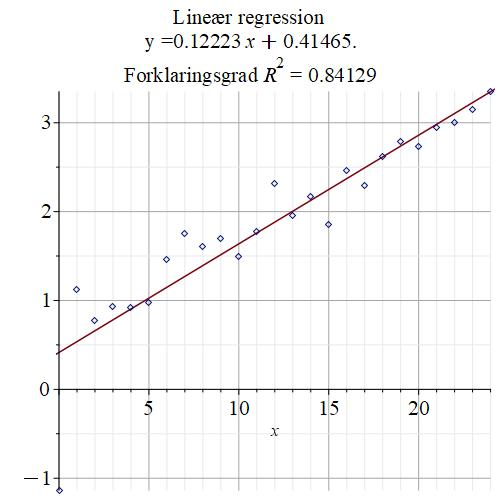
\includegraphics[width=0.7\textwidth]{Billeder/bakterielinreg.jpg}
		\caption{Lineær regression i enkeltlogaritmisk koordinatsystem}
		\label{fig:linlogreg}
	\end{figure}
	Den lineære model lyder
	\begin{align*}
		\ln(y) = 0.12223x+0.41465.
	\end{align*}
	Ønsker vi at bestemme den eksponentielle sammenhæng ud fra dette data, så skal vi transformere koefficienterne tilbage som det fremgår af \eqref{enkeltlog}.
	Vi får derfor, at 
	\begin{align*}
		b = e^{0.41465} = 1.5138
	\end{align*}
	og
	\begin{align*}
		a = e^{0.12223} = 1.1300,
	\end{align*}
	og den eksponentielle sammenhæng mellem den forløbne tid $x$ og antallet af bakterier $y$ er derfor
	\begin{align*}
		y = 1.5138\cdot 1.13^x,
	\end{align*}
	hvilket er nøjagtigt hvad vi bestemte ved den eksponentielle regression. Der er dog værd at notere, at det formentlig er præcist sådan at Maple laver eksponentiel 
	regression, og derfor er det heller ikke mærkeligt, at vi opnår det samme resultat.
\end{exa}

\section*{Opgave 1}

I \href{https://github.com/ChristianJLex/TeachingNotes/raw/master/2022-2023/Data%20og%20lign/logBakterier.xlsx}{\color{blue!60}dette datasæt} fremgår sammenhængen mellem antal forløbne minutter $x$ og $ln(y)$, hvor $y$ er antallet af bakterier i en bestemt opløsning. 
Det antages, at der er lineær sammenhæng mellem $x$ og $\ln(y)$. 
\begin{enumerate}[label=\roman*)]
	\item Brug datasættet til at bestemme en sammenhæng 
	\begin{align*}
		\ln(y) = ax + b.
	\end{align*}
	\item Afgør, om residualerne er normalfordelte og brug dette til at afgøre, om modellen er god.
	\item Brug din model til at bestemme en ligning for den eksponentielle sammenhæng
	\begin{align*}
		y = \beta \cdot \alpha^x.
	\end{align*}
	\item Brug din model til at afgøre, hvornår der vil være 1 bio. bakterier i opløsningen. 
\end{enumerate}

\section*{Opgave 2}

Man har målt 10 forskellige bremselængder for 10 forskellige biler med omtrent samme vægt ved tilfældigt udvalgte hastigheder. I \href{https://github.com/ChristianJLex/TeachingNotes/raw/master/2022-2023/Data%20og%20lign/logBremselaengde.xlsx}{\color{blue!60}dette datasæt} kan $\ln(x)$ og 
$\ln(y)$ findes, hvor $x$ er hastigheden af bilen (i m/s) og $y$ er bremselængden (i meter). Vi antager, at der er en potenssammenhæng mellem $x$ og $y$.

\begin{enumerate}[label=\roman*)]
	\item Brug datasættet til at bestemme en sammenhæng 
	\begin{align*}
		\ln(y) = \ln(b) +a\ln(x).
	\end{align*}
	\item Afgør, om residualerne er normalfordelte og brug dette til at afgøre, om modellen er god.
	\item Brug din model til at bestemme en ligning for potenssammenhængen
	\begin{align*}
		y = \beta \cdot x^\alpha.
	\end{align*}
	\item Brug din model til at bestemme bremselængden for en bil, der kører 100m/s.
\end{enumerate}
